\documentclass[12pt,a4paper]{article}
\usepackage[utf8]{inputenc}
\usepackage[german]{babel}
\usepackage[T1]{fontenc}
\usepackage{amsmath}
\usepackage{amsfonts}
\usepackage{amssymb}
\usepackage{graphicx}
\usepackage{siunitx}
\usepackage[left=2cm,right=2cm,top=2cm,bottom=2cm]{geometry}
\author{Tim}

\begin{document}
\sisetup{separate-uncertainty = true}
	\setlength{\parindent}{0pt} 
	\begin{center}
		{\LARGE Versuchsprotokoll}\\
		\begin{large}
			zum Grundpraktikum Physik Teil II\\[0.4cm]
			an der RWTH Aachen\\
			I. Physikalisches Institut B\\[4.5cm]
			\Large\textbf{\textsl{E-Lehre}}\\[4cm]
			\normalsize\textit{vorgelegt\\von}\\[0.4cm]
			\large{Moritz Berger\\Tim Herbermann\\Gerald Kolter\\Sebastian Siebert}\\[1cm]
			\large \textit{Gruppe A07} \\ [3cm]
			\large \textbf{Sommersemester 2017}
		\end{large}
	\end{center}
	\newpage
	
	\tableofcontents
	\newpage


\section{Grundlagen}

\subsection{Versuchsbeschreibung}
In den folgenden Versuchen wurde die Güte von Serien- und Parallelschwingkreisen auf verschiedene Arten bestimmt. Zusätzlich wurde in einem letzten Aufbau ein Hoch- bzw. Tiefpass untersucht.

\subsection{Physikalische Grundlagen}

\paragraph{Serienkreis}
Aus der Kirchhoffschen Maschenregel ergibt sich eine Differentialgleichung zur Beschreibung der erzwungenen Schwingung.

\begin{equation}
\frac{U}{L} = \frac{d^2 Q}{dt^2}+\frac{R}{L}\frac{dQ}{dt}+\frac{1}{LC} Q
\end{equation}



Dabei ergibt sich der maximale Strom im Kreis bei Resonanz für
\begin{equation}
\omega_0 = \frac{1}{\sqrt{LC}}
\end{equation} 

Die Güte des Schwingkreises ist definiert durch
\begin{equation}
Q_s = \frac{1}{R} \sqrt{\frac{L}{C}}
\label{equ:Guete_Bauteile_Groesse}
\end{equation}

und beschreibt unter anderem den Zusammenhang zwischen angelegter Spannung und Spannungsüberhöhung im Resonanzfall:

\begin{equation}
\frac{U_L(\omega_0)}{U(\omega_0)} = Q_s 
\label{equ:Guete_Spannungsüberhöhung}
\end{equation}

Man stellt fest, dass die Güte sich auch noch als Quotient aus Resonanzfrequenz und Breite der Resonanzkurve bestimmen lässt:
\begin{equation}
\dfrac{\omega_0}{\Delta \omega} = \dfrac{\omega_0}{2d} = \dfrac{\omega_0 L}{R} = \dfrac{1}{R \omega_0 L} = \dfrac{1}{R} \cdot \sqrt{\dfrac{L}{C}} =: Q_S
\label{equ:Guete_Resonanzbreite}
\end{equation}

Die Resonanzfrequenz und die Breite der Resonanzkurve können dazu auf 2 verschiedene Arten bestimmt werden:\\
Die Resonanzfrequenz liegt vor, wenn der Strom im Serienschwingkreis als Funktion der Frequenz sein Maximum erreicht. Die Breite der Resonanzkurve wird durch die beiden Punkte bestimmt, bei denen der Strom auf $\frac{I_{max}}{\sqrt{2}}$ abgefallen ist.\\
Im Fall der Resonanzfrequenz gilt für die Phasenverschiebung $\phi$ zwischen Strom und Spannung $\phi = 0$. Die Breite wird durch die beiden Punkte bestimmt, bei denen die Phasenverschiebung $\phi = \pm \ang{45}$ ist.



\paragraph{Parallelschwingkreis}
Aus der Knotenregel kann ebenfalls eine Differentialgleichung zur Beschreibung des Parallelschwingkreises hergeleitet werden.

Aus dieser kann ebenfalls die Resonanzfrequenz bestimmt werden.

\begin{equation}
\omega_0 = \sqrt{\frac{1-\frac{C}{L}\cdot R_L^2}{LC}}
\end{equation} 

Für große Widerstände im Kreis ergibt sich für die Güte der Schaltung näherungsweise der Zusammenhang:

\begin{equation}
Q_P = \frac{1}{R_L} \sqrt{\frac{L}{C}}
\label{equ:Güte_Bauteile}
\end{equation}

Im Falle des Parallelschwingkreises kommt es bei Resonanz zu einer Stromüberhöhung. Auch hier ergibt sich der Zusammenhang:

\begin{equation}
\frac{(I_L)_0}{I_0} = Q_p
\label{eq:Parallel_Strmhoch}
\end{equation}

Auch beim Parallelschwingkreis kann die Güte aus der Resonanzfrequenz und der Breite der Resonanzkurve bestimmt werden. Bestimmt werden diese dann aus der Spannung, die am Kreis anliegt und nicht aus dem Strom. Die Bestimmung von Resonanzfrequenz und Breite der Resonanzkurve ist dabei analog zu der beim Serienkreis. Die Berechnung der Güte daraus ist analog zu Gl. \ref{equ:Guete_Resonanzbreite}.


\paragraph{Hoch -und Tiefpass}
Ein Hoch- bzw. Tiefpass 1. Ordnung besteht aus einer Serienschaltung von Widerstand und Kondensator. Durch Anlegen einer Wechselspannung werden, abhängig davon wo die Spannung abgegriffen wird, entweder große oder kleine Frequenzen blockiert bzw. durchgelassen.

Der Hochpass ergibt sich durch Spannungsabgriff am Widerstand. Die Übertragungsfunktion ergibt sich dabei zu:

\begin{equation}
\frac{U_a}{U_e} = \frac{1}{\sqrt{\left(\frac{1}{\omega C R}\right)^2+1}}
\end{equation}

Den Tiefpass erhält man dann entsprechend durch Abgriff am Kondensator. Die Übertragungsfunktion lautet:

\begin{equation}
\frac{U_a}{U_e} = \frac{1}{\sqrt{1+(\omega C R)^2}}
\end{equation}

\section{Serienschwingkreis}

\subsection{Aufbau und Durchführung}

\begin{figure}
\centering
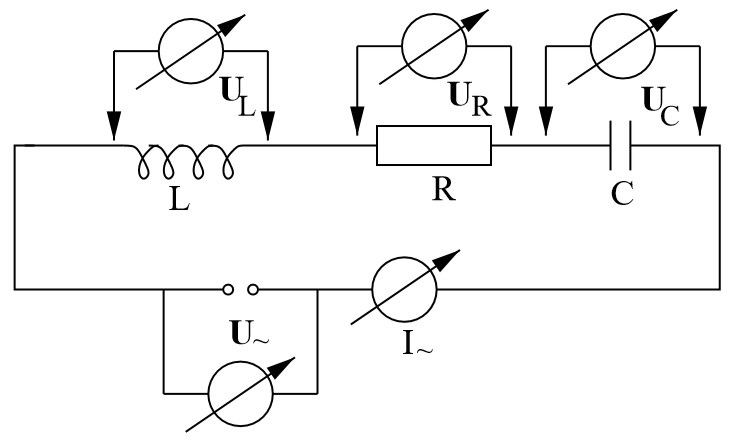
\includegraphics[scale=0.8]{Bilder/AufbauSerie.png}
\caption{Schaltbild zum Serienschwingkreis. Die Spannungsmessung am Ohmschen Widerstand wurde nur im Rahmen der Vorauswertung mit dem Oszilloskop durchgeführt.}
\label{fig:AufbauSerie}
\end{figure}

Der wesentliche Versuchsaufbau ist in Abbildung \ref{fig:AufbauSerie} gezeigt. Für alle Versuche zum Serienkreis wurde der Kondensator mit Nominalkapazität $C=\SI{4,7}{\micro \F}$ und die Spule mit 250 Windungen verwendet.

Die Messung der Spannung am Ohmschen Widerstand findet dabei nur im Rahmen des Vorversuches mit einem Oszilloskop statt.
Im Hauptversuch werden Gesamtspannung und Strom über das Power-CASSY, welches gleichzeitig als Spannungsquelle fungiert, als Effektivwerte gemessen. Die abfallenden Spannungen an Spule und Kondensator werden mit dem Sensor-CASSY ebenfalls als Effektivwerte aufgezeichnet. Der Messvorgang wird mit verschiedenen Widerständen wiederholt.

Die am Power-CASSY eingestellte Wechselspannungsamplitude wurde abhängig vom Widerstand gewählt. Der Gleichspannungsoffset beträgt $U = \SI{0}{V}$. Die Signalform ist eine Sinusschwingung.

Die Frequenz wurde automatisch über die Formel $f_1 = f_0 +(n-1) \cdot \Delta f$ automatisch variiert. Über eine die Zusatzbedingung der Form$f_1 < f_{Grenz}$ and $\Delta t > 2$ wurde ein Abbruch bei einer maximalen Frequenz sowie das Aufzeichnen des Messwertes nach dem Einschwingvorgang gewährleistet. Der Messbereich der Spannung ist 0-7V. Start- und Endfrequenz wurden dabei für jeden Widerstand unterschiedlich gewählt.

\subsection{Vorauswertung: Oszilloskop}
Im Rahmen der Vorauswertung wurde die Spannung am Ohmschen Widerstand und die gesamte abfallende Spannung mittels Oszilloskop gemessen. Für beide Gruppen wurde der Widerstand mit Nominalwert $R = 5,1 \Omega$ verwendet. Die Frequenz der angelegten Wechselspannung wird über den Frequenzgenerator eingestellt.\\

Zur Bestimmung der Resonanzfrequenz werden die gemessenen Spannungen an beiden Kanälen im Oszilloskop gegeneinander aufgetragen. Die Frequenz wurde so eingestellt, dass die Ellipse verschwindet und die Spannungswerte eine Gerade bilden. Der entsprechende Frequenzwert ist die Resonanzfrequenz
Zur Bestimmung der Resonanzbreite werden in der Zeitdarstellung des Oszilloskops diejenigen Frequenzen bestimmt, für die die Amplitude der Spannung am Widerstand um den Faktor $\sqrt{2}$ kleiner als im Resonanzfall ist. 

Es gilt

\begin{equation}
\Delta f = f_2 - f_1 \quad \Rightarrow \quad Q = \frac{f_0}{\Delta f}
\end{equation}

und mittels Fehlerfortpflanzung:

\begin{equation}
\sigma_{\Delta f} = \sqrt{\sigma_{f_1}^2+\sigma_{f_2}^2} \qquad \sigma_Q = Q \sqrt{\left(\frac{\sigma_{f_0}}{f_0}\right)^2 + \left(\frac{\sigma_{\Delta f}}{\Delta f}\right)^2}
\end{equation}

Die Ergebnisse der Voruntersuchung sind für beide Gruppen in Tabelle \ref{tab:Voruntersuchung} dargestellt.

\begin{table}
\centering
\begin{tabular}{|c|c|c|c|c|}
\hline
Gruppe & $f$/Hz & $f_1$/Hz & $f_2$/Hz & Q\\
\hline
A & $2094 \pm 3$ & $1781 \pm 6$ & $2510 \pm 6$ & $2.87 \pm 0.03$ \\
\hline
B & $2149 \pm 2$ & $1755 \pm 4$ & $2614 \pm 4$ & $2.50 \pm 0.02$\\
\hline
\end{tabular}
\caption{Ergebnisse der Voruntersuchung mittels Oszilloskop}
\label{tab:Voruntersuchung}
\end{table}


Eine zweite Voruntersuchung durch Bestimmen der Spannungsüberhöhung im Resonanzfall war aus Zeitgründen nicht möglich.

\subsection{Auswertung}
Zur Bestimmung der Güte eines Serienschwingkreises gibt es die folgenden 4 Möglichkeiten:
\begin{enumerate}
\item Man misst die Resonanzfrequenz und die Breite der Resonanzkurve. Die Güte ist dann gemäß Gl. \ref{equ:Guete_Resonanzbreite} der Quotient aus beiden.
\item Ein analoges Verfahren lässt sich mit der Phasenverschiebung durchführen: Die Resonanzfrequenz ist dann bei $\varphi = 0$ und die Breite $\Delta \omega$ ist zwischen $\varphi = \pm \ang{45}$.
\item Gemäß Gl. \ref{equ:Guete_Spannungsüberhöhung} lässt sich die Güte auch aus der Spannungsüberhöhung an der Resonanzfrequenz bestimmen.
\item Mit Gl. \ref{equ:Guete_Bauteile_Groesse} kann die Güte aus den Größen der Bauteilen berechnet werden.
\end{enumerate}

\paragraph{Gruppe A}
Für die Auswertungsmöglichkeiten 1-3 wurden die jeweiligen Werte jeweils abgelesen und automatisiert berechnet.\\
Die automatisiert berechneten Werte gehen über die einzelnen Messpunkte. Dabei werden Schnittpunkte immer als der Mittelwert der beiden Messpunkte, zwischen denen der Schnittpunkt liegt, approximiert. Für die Bestimmung des Fehlers auf diese Berechnung wird eine Gleichverteilung angenommen.\\


\subsubsection{Resonanzfrequenz und Breite der Resonanzkurve}

% Plots Gruppe A
\begin{figure}
	\centering
	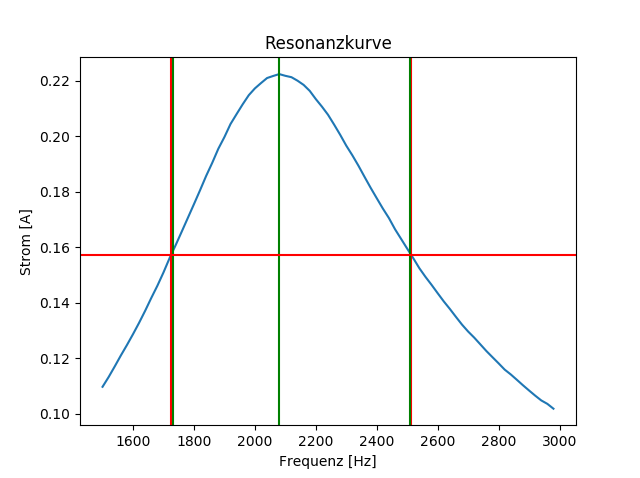
\includegraphics[scale=0.8]{Bilder/Serie_Resonanzkurve_A_5.png}
	\caption{Resonanzkurve des Aufbaus A mit $\SI{5}{\ohm}$ Widerstand. Die waagerechte Linie markiert die Stelle bei der $I = \frac{I_{max}}{\sqrt{2}}$ gilt. Die senkrechten Linien sind die Auswertungslinien (rot = abgelesen, grün = automatisiert ausgerechnet).}
	\label{fig:Serie_Resonanzkurve_A_5}
\end{figure}
\begin{figure}
	\centering
	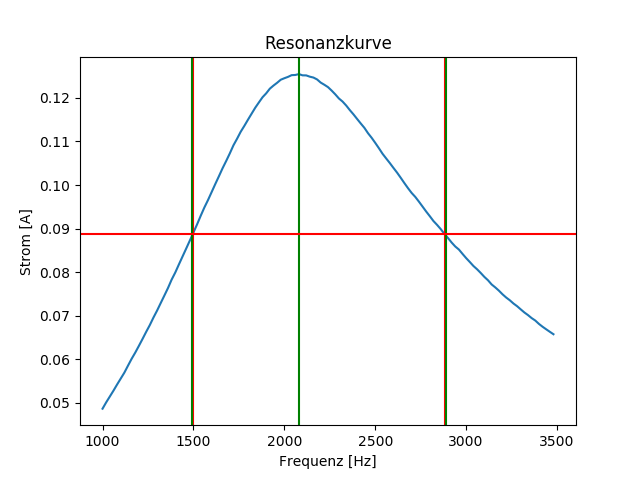
\includegraphics[scale=0.8]{Bilder/Serie_Resonanzkurve_A_10.png}
	\caption{Resonanzkurve des Aufbaus A mit $\SI{10}{\ohm}$ Widerstand. Die waagerechte Linie markiert die Stelle bei der $I = \frac{I_{max}}{\sqrt{2}}$ gilt. Die senkrechten Linien sind die Auswertungslinien (rot = abgelesen, grün = automatisiert ausgerechnet).}
	\label{fig:Serie_Resonanzkurve_A_10}
\end{figure}


% Plots Gruppe B
\begin{figure}
	\centering
	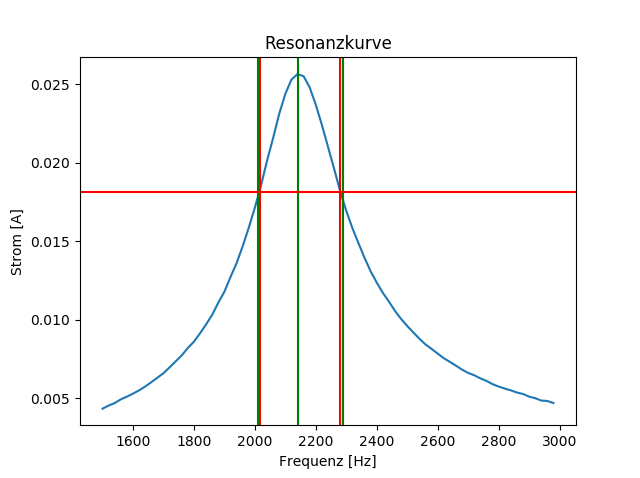
\includegraphics[scale=0.8]{Bilder/Serie_Resonanzkurve_B_1.png}
	\caption{Resonanzkurve des Aufbaus B mit $\SI{1}{\ohm}$ Widerstand. Die waagerechte Linie markiert die Stelle bei der $I = \frac{I_{max}}{\sqrt{2}}$ gilt. Die senkrechten Linien sind die Auswertungslinien (rot = abgelesen, grün = automatisiert ausgerechnet).}
	\label{fig:Serie_Resonanzkurve_B_1}
\end{figure}
\begin{figure}
	\centering
	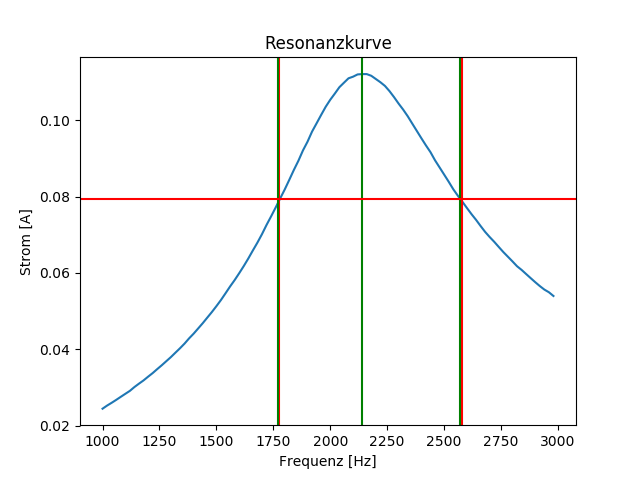
\includegraphics[scale=0.8]{Bilder/Serie_Resonanzkurve_B_5.png}
	\caption{Resonanzkurve des Aufbaus B mit $\SI{5}{\ohm}$ Widerstand. Die waagerechte Linie markiert die Stelle bei der $I = \frac{I_{max}}{\sqrt{2}}$ gilt. Die senkrechten Linien sind die Auswertungslinien (rot = abgelesen, grün = automatisiert ausgerechnet).}
	\label{fig:Serie_Resonanzkurve_B_5}
\end{figure}
\begin{figure}
	\centering
	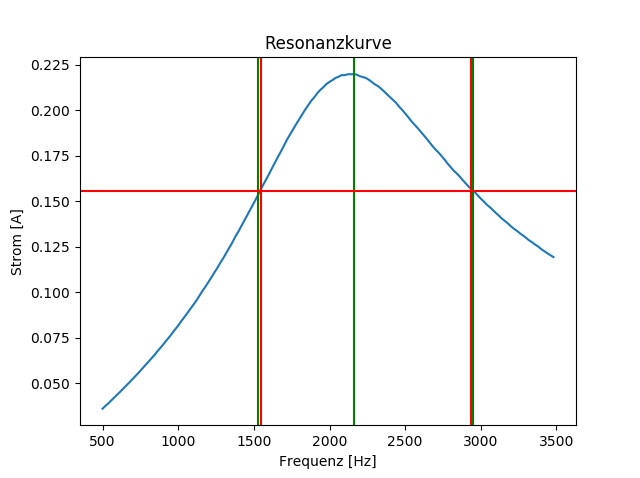
\includegraphics[scale=0.8]{Bilder/Serie_Resonanzkurve_B_10.png}
	\caption{Resonanzkurve des Aufbaus B mit $\SI{10}{\ohm}$ Widerstand. Die waagerechte Linie markiert die Stelle bei der $I = \frac{I_{max}}{\sqrt{2}}$ gilt. Die senkrechten Linien sind die Auswertungslinien (rot = abgelesen, grün = automatisiert ausgerechnet).}
	\label{fig:Serie_Resonanzkurve_B_10}
\end{figure}



In den Abbildungen \ref{fig:Serie_Resonanzkurve_A_5} und \ref{fig:Serie_Resonanzkurve_A_10} sind die Resonanzkurven von Gruppe A mit dem $\SI{5}{\ohm}$ und dem $\SI{10}{\ohm}$ Widerstand dargestellt. \\
Abbildungen \ref{fig:Serie_Resonanzkurve_B_1}, \ref{fig:Serie_Resonanzkurve_B_5} und \ref{fig:Serie_Resonanzkurve_B_10} zeigen die Resonanzkurven für die Aufbauten von Gruppe B mit den $\SI{1}{\ohm}$, $\SI{5}{\ohm}$ und $\SI{10}{\ohm}$ Widerständen.

\begin{table}
	\centering
	\begin{tabular}{|c|c|c|c||c|c|c|}
		\hline
		Widerstand & $f_0$/Hz & $f_1$/Hz & $f_2$/Hz & $f_0$/Hz & $f_1$/Hz & $f_2$/Hz \\
		\hline
		&&&&&&\\
		Gruppe A &&&&&&\\
		\hline
		$\SI{5}{\ohm}$ & 2080 & 1724 & 2513 & 2080 & 1730 & 2510 \\
		\hline
		$\SI{10}{\ohm}$ & 2080 & 1496 & 2882 & 2080 & 1490 & 2890 \\
		\hline
		&&&&&&\\
		Gruppe B &&&&&&\\
		\hline
		\SI{1}{\ohm} & 2140 & 2016 & 2278 & 2140 & 2010 & 2290 \\
		\hline
		\SI{5}{\ohm} & 2040 & 1776 & 2578 & 2040 & 1770 & 2570 \\
		\hline
		\SI{10}{\ohm} & 2040 & 1549 & 2933 & 2040 & 1530 & 2950 \\
		\hline
	\end{tabular}
	\caption{Erhaltene Frequenzen der Resonanzkurve des Stroms im Serienschwingkreis. Links sind die abgelesenen Werte, rechts die automatisiert berechneten.}
	\label{tab:StromResonanz}
\end{table}


Tabelle \ref{tab:StromResonanz} zeigt die abgelesenen und automatisiert berechneten Werte für die Resonanzfrequenz $f_0$ und die beiden die Resonanzbreite begrenzenden Frequenzen $f_1$ und $f_2$. Auffällig ist, dass die Resonanzfrequenz beim Ablesen und bei der automatisierten Auswertung identisch ist. Dies liegt daran, dass die Resonanzkurve durch die geringe Punktdichte eine klare Spitze aufweist, weil es einen größten Messpunkt gibt. Daher ist der abgelesene Wert zwangsweise identisch mit dem Maximum.



Die Unsicherheit bei der automatisierten Rechnung wird mit dem Abstand zweier Messpunkte bei Annahme einer Gleichverteilung angegeben:
\begin{equation*}
\sigma_{f_{berechnet}} = \dfrac{\SI{20}{Hz}}{\sqrt{12}}
\end{equation*}

Die Unsicherheit beim Ablesen wird mit 
\begin{equation*}
\sigma_{f_{abgelesen}} = \SI{5}{Hz}
\end{equation*}
abgeschätzt.\\

Die Fehlerfortpflanzung ist für die Auswertung durch Ablesen und die automatisierte Auswertung identisch:\\
Nach Gl. \ref{equ:Guete_Resonanzbreite} pflanzt sich der Fehler auf die Frequenz fort:
\begin{equation}
\dfrac{\sigma_Q}{Q} = \sqrt{\left( \dfrac{\sigma_f}{f_0} \right)^2 + \left( \dfrac{\sigma_{\Delta f}}{\Delta f} \right)^2} = \sqrt{\left( \dfrac{\sigma_f}{f_0} \right)^2 + \left( \dfrac{\sqrt{2} \cdot \sigma _f}{\Delta f} \right)^2}
\label{equ:FehlerGuete_FehlerFrequenz}
\end{equation}

Damit ergibt sich aus dieser Methode die Güte des Schwingkreises mit Gl. \ref{equ:Guete_Resonanzbreite} und Gl. \ref{equ:FehlerGuete_FehlerFrequenz} zu den in Tabelle \ref{tab:Serienguete_Var1} zusammengefassten Werten.

\begin{table}
	\centering
	\begin{tabular}{|c|c|c|}
		\hline
		Widerstand & Q\textsubscript{abgelesen} & Q\textsubscript{berechnet} \\
		\hline
		&&\\
		Gruppe A &&\\
		\hline
		\SI{5}{\ohm} & \num{2.639(25)} & \num{2.667(29)} \\
		\hline
		\SI{10}{\ohm} & \num{1.500(9)} & \num{1.486(10)} \\
		\hline
		&&\\
		Gruppe B &&\\
		\hline
		\SI{1}{\ohm} & \num{8.17(22)} & \num{7.64(22)} \\
		\hline
		\SI{5}{\ohm} & \num{2.675(28)} & \num{2.668(24)} \\
		\hline
		\SI{10}{\ohm} & \num{1.561(9)} & \num{1.521(10)} \\
		\hline		
	\end{tabular}
	\caption{Ergebnisse der Gütebestimmung durch die Breite der Stromkurve}
	\label{tab:Serienguete_Var1}
\end{table}

\subsubsection{Phasenverschiebung}

Die Verläufe der Phasenverschiebung in Abhängigkeit von der Frequenz der angelegten Spannung ist für die verschiedenen Aufbauten in Abbildungen \ref{fig:Serie_Phasenverschiebung_A_5} bis \ref{fig:Serie_Phasenverschiebung_B_10} dargestellt.


% Gruppe A
\begin{figure}
	\centering
	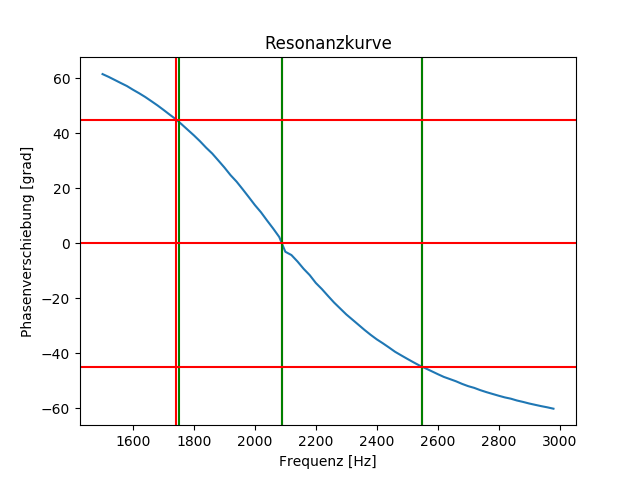
\includegraphics[scale=0.8]{Bilder/Serie_Phasenverschiebung_A_5.png}
	\caption{Phasenverschiebung des Aufbaus A mit \SI{5}{\ohm} Widerstand. Die waagerechten Linien markieren die Stellen bei der $\varphi = \ang{0}, \pm \ang{45}$. Die senkrechten Linien sind die Auswertungslinien (rot = abgelesen, grün = automatisiert ausgerechnet).}
	\label{fig:Serie_Phasenverschiebung_A_5}
\end{figure}
\begin{figure}
	\centering
	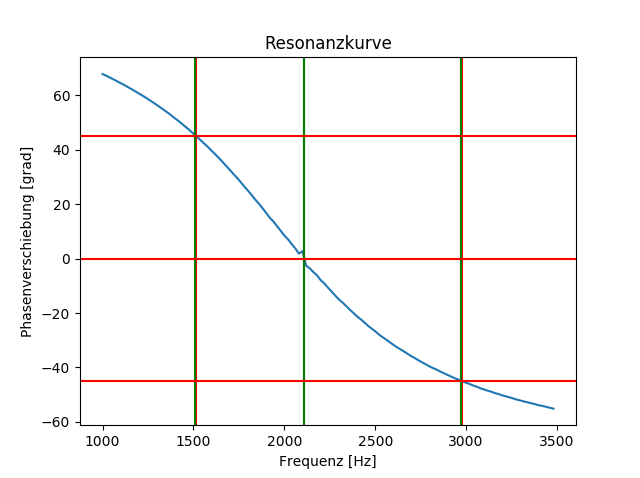
\includegraphics[scale=0.8]{Bilder/Serie_Phasenverschiebung_A_10.png}
	\caption{Phasenverschiebung des Aufbaus A mit \SI{10}{\ohm} Widerstand. Die waagerechten Linien markieren die Stellen bei der $\varphi = 0, \pm \ang{45}$ ist. Die senkrechten Linien sind die Auswertungslinien (rot = abgelesen, grün = automatisiert ausgerechnet).}
	\label{fig:Serie_Phasenverschiebung_A_10}
\end{figure}

% Gruppe B
\begin{figure}
	\centering
	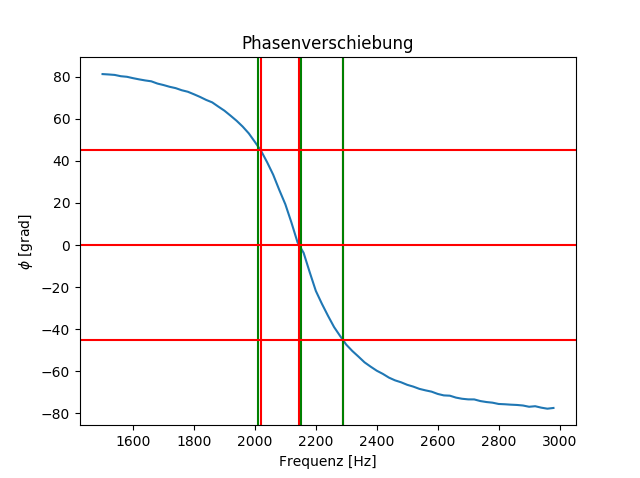
\includegraphics[scale=0.8]{Bilder/Serie_Phasenverschiebung_B_1.png}
	\caption{Phasenverschiebung des Aufbaus B mit \SI{1}{\ohm} Widerstand. Die waagerechten Linien markieren die Stellen bei der $\varphi = \ang{0}, \pm \ang{45}$ ist. Die senkrechten Linien sind die Auswertungslinien (rot = abgelesen, grün = automatisiert ausgerechnet).}
	\label{fig:Serie_Phasenverschiebung_B_1}
\end{figure}
\begin{figure}
	\centering
	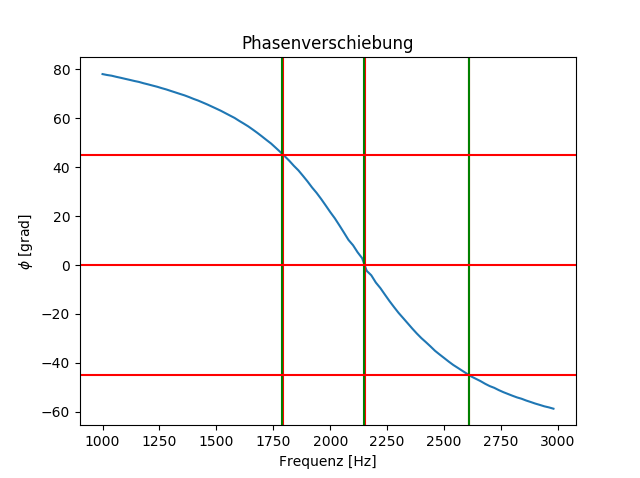
\includegraphics[scale=0.8]{Bilder/Serie_Phasenverschiebung_B_5.png}
	\caption{Phasenverschiebung des Aufbaus B mit \SI{5}{\ohm} Widerstand. Die waagerechten Linien markieren die Stellen bei der $\varphi = \ang{0}, \pm \ang{45}$. Die senkrechten Linien sind die Auswertungslinien (rot = abgelesen, grün = automatisiert ausgerechnet).}
	\label{fig:Serie_Phasenverschiebung_B_5}
\end{figure}
\begin{figure}
	\centering
	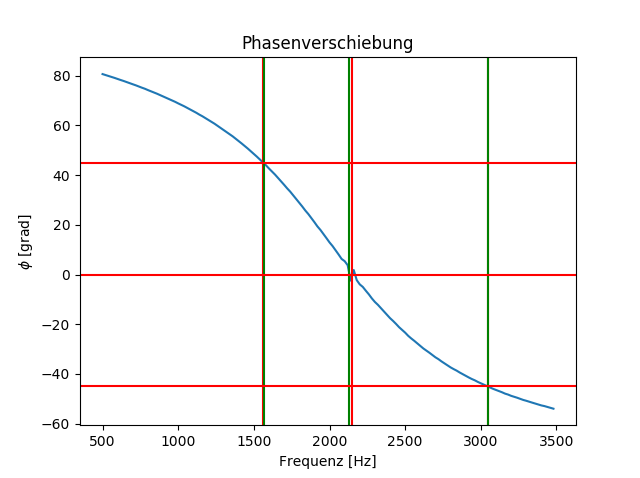
\includegraphics[scale=0.8]{Bilder/Serie_Phasenverschiebung_B_10.png}
	\caption{Phasenverschiebung des Aufbaus B mit \SI{10}{\ohm} Widerstand. Die waagerechten Linien markieren die Stellen bei der $\varphi = \ang{0}, \pm \ang{45}$ ist. Die senkrechten Linien sind die Auswertungslinien (rot = abgelesen, grün = automatisiert ausgerechnet).}
	\label{fig:Serie_Phasenverschiebung_B_10}
\end{figure}



Tabelle \ref{tab:StromPhasenverschiebung} zeigt die abgelesenen und automatisiert berechneten Werte für die Resonanzfrequenz $f_1$ und die beiden die Resonanzbreite begrenzenden Frequenzen $f_1$ und $f_2$.


\begin{table}
	\centering
	\begin{tabular}{|c|c|c|c||c|c|c|}
		\hline
		Widerstand & $f_0$/Hz & $f_1$/Hz & $f_2$/Hz & $f_0$/Hz & $f_1$/Hz & $f_2$/Hz \\
		\hline
		&&&&&&\\
		Gruppe A &&&&&&  \\
		\hline
		\SI{5}{\ohm} & 2088 & 1742 & 2550 & 2090 & 1750 & 2550 \\
		\hline
		\SI{10}{\ohm} & 2110 & 1516 & 2976 & 2110 & 1510 & 2970 \\
		\hline
		&&&&&&\\
		Gruppe B &&&&&&\\
		\hline
		\SI{1}{\ohm} & 2145 & 2019 & 2288 & 2150 & 2010 & 2290 \\
		\hline
		\SI{5}{\ohm} & 2151 & 1793 & 2609 & 2150 & 1790 & 2610 \\
		\hline
		\SI{10}{\ohm} & 2139 & 1549 & 2933 & 2130 & 1570 & 3050 \\
		\hline
	\end{tabular}
	\caption{Frequenzen zur Phasenverschiebung im Serienschwingkreis. Links sind die abgelesenen Werte, rechts die automatisiert berechneten.}
	\label{tab:StromPhasenverschiebung}
\end{table}


Die automatisierte Auswertung wurde genauso realisiert wie bei Methode 1. \\
Die Fehlerrechnung kann komplett aus der Auswertung nach der ersten Methode übernommen werden (siehe Gl. \ref{equ:FehlerGuete_FehlerFrequenz}).

Damit ergibt sich aus dieser Methode die Güte des Schwingkreises mit Gl. \ref{equ:Guete_Resonanzbreite} und Gl. \ref{equ:FehlerGuete_FehlerFrequenz}. Die Werte sind in Tabelle \ref{tab:Serienguete_Var2} zusammengefasst.


\begin{table}
	\centering
	\begin{tabular}{|c|c|c|}
		\hline
		Widerstand &  Q\textsubscript{abgelesen} & Q\textsubscript{berechnet} \\
		\hline
		&&\\
		Gruppe A &&\\
		\SI{5}{\ohm} & \num{2.586(24)} & \num{2.613(28)} \\
		\hline
		\SI{10}{\ohm} & \num{1.446(8)} & \num{1.445(9)} \\
		\hline
		&&\\
		Gruppe B &&\\
		\hline
		\SI{1}{\ohm} & \num{7.97(21)} & \num{7.68(22)} \\
		\hline
		\SI{5}{\ohm} & \num{2.636(24)} & \num{2.622(27)} \\
		\hline
		\SI{10}{\ohm} & \num{1.443(8)} & \num{1.439(9)} \\
		\hline
	\end{tabular}
	\caption{Ergebnisse der Gütebestimmung durch die Phasenverschiebung.}
	\label{tab:Serienguete_Var2}
\end{table}



\subsubsection{Spannungsüberhöhung}
% Gruppe A
\begin{figure}
	\centering
	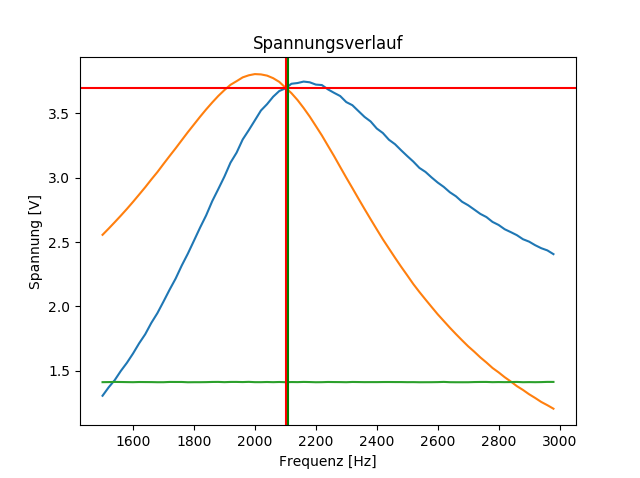
\includegraphics[scale=0.8]{Bilder/Serie_Spannungsueberhoehung_A_5.png}
	\caption{Verlauf der Kondensator- (orange), Spulen- (blau) und angelegten Spannung (grün) beim Aufbau A mit dem $\SI{5}{\ohm}$ Widerstand. Die waagerechte Linie markiert den Spannungswert des Schnittpunktes und die senkrechten Linien die zugehörige Frequenz (rot = abgelesen, grün = automatisiert ausgerechnet).}
	\label{fig:Serie_Spannungsueberhoehung_A_5}
\end{figure}
\begin{figure}
	\centering
	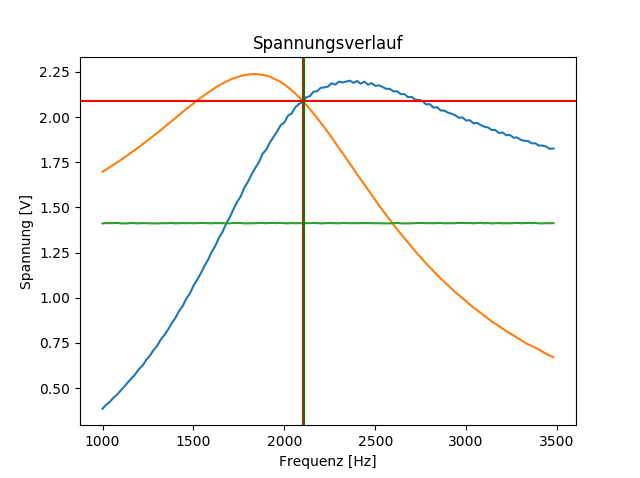
\includegraphics[scale=0.8]{Bilder/Serie_Spannungsueberhoehung_A_10.png}
	\caption{Verlauf der Kondensator- (orange), Spulen- (blau) und angelegten Spannung (grün) beim Aufbau A mit dem $\SI{10}{\ohm}$ Widerstand. Die waagerechte Linie markiert den Spannungswert des Schnittpunktes und die senkrechten Linien die zugehörige Frequenz (rot = abgelesen, grün = automatisiert ausgerechnet).}
	\label{fig:Serie_Spannungsueberhoehung_A_10}
\end{figure}


% Gruppe B
\begin{figure}
	\centering
	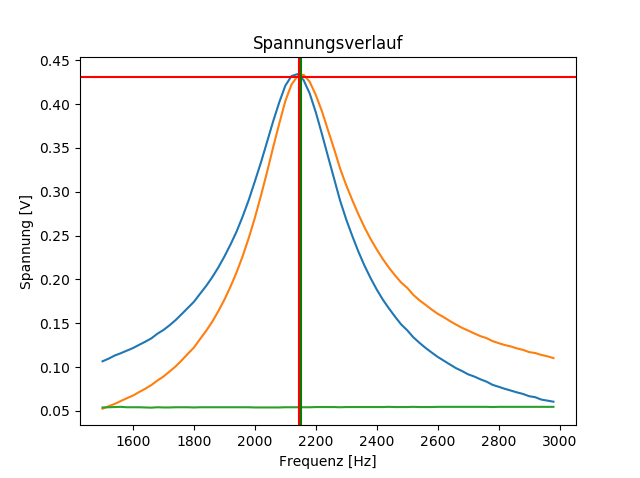
\includegraphics[scale=0.8]{Bilder/Serie_Spannungsueberhoehung_B_1.png}
	\caption{Verlauf der Kondensator- (orange), Spulen- (blau) und angelegten Spannung (grün) beim Aufbau B mit dem $\SI{1}{\ohm}$ Widerstand. Die waagerechte Linie markiert den Spannungswert des Schnittpunktes und die senkrechten Linien die zugehörige Frequenz (rot = abgelesen, grün = automatisiert ausgerechnet).}
	\label{fig:Serie_Spannungsueberhoehung_B_1}
\end{figure}
\begin{figure}
	\centering
	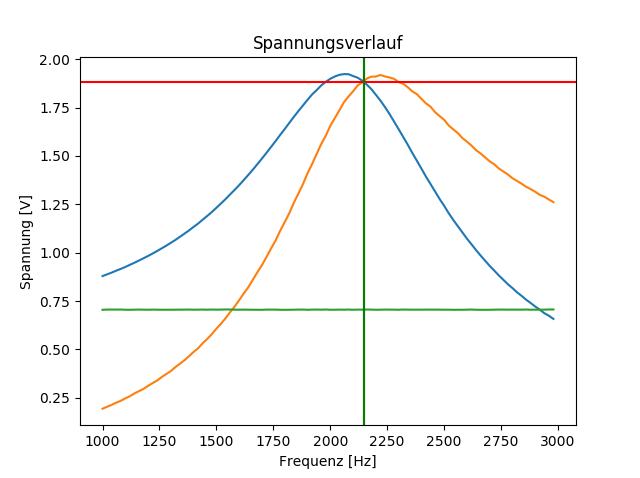
\includegraphics[scale=0.8]{Bilder/Serie_Spannungsueberhoehung_B_5.png}
	\caption{Verlauf der Kondensator- (orange), Spulen- (blau) und angelegten Spannung (grün) beim Aufbau B mit dem $\SI{5}{\ohm}$ Widerstand. Die waagerechte Linie markiert den Spannungswert des Schnittpunktes und die senkrechten Linien die zugehörige Frequenz (rot = abgelesen, grün = automatisiert ausgerechnet).}
	\label{fig:Serie_Spannungsueberhoehung_B_5}
\end{figure}
\begin{figure}
	\centering
	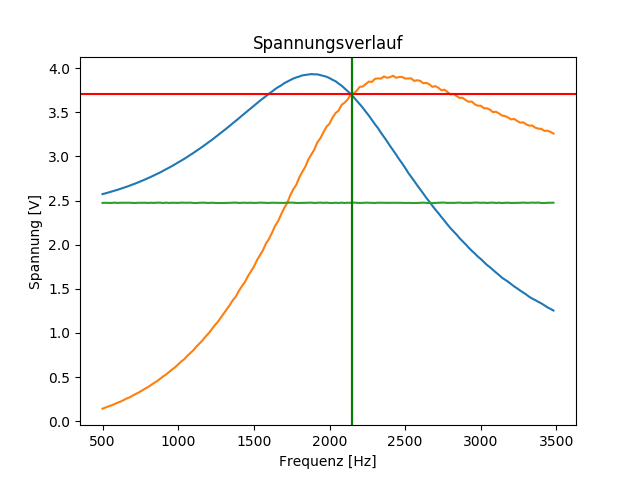
\includegraphics[scale=0.8]{Bilder/Serie_Spannungsueberhoehung_B_10.png}
	\caption{Verlauf der Kondensator- (orange), Spulen- (blau) und angelegten Spannung (grün) beim Aufbau B mit dem $\SI{10}{\ohm}$ Widerstand. Die waagerechte Linie markiert den Spannungswert des Schnittpunktes und die senkrechten Linien die zugehörige Frequenz (rot = abgelesen, grün = automatisiert ausgerechnet).}
	\label{fig:Serie_Spannungsueberhoehung_B_10}
\end{figure}




\begin{table}
	\centering
	\begin{tabular}{|c|c|c|c||c|c|c|}
		\hline
		Widerstand & $f_0$/Hz & $U_{L, f_0}$/V & $U_{an, f_0}$/V & $f_0$/Hz & $U_{L, f_0}$/V & $U_{an, f_0}$/V \\
		\hline
		&&&&&&\\
		Gruppe A &&&&&&\\
		\hline
		\SI{5}{\ohm} & 2102 & 3.6964 & 1.4123 & 2110 & 3.7114 & 1.4122 \\
		\hline
		\SI{10}{\ohm} & 2103 & 2.0867 & 1.4123 & 2110 & 2.0967 & 1.4122 \\
		\hline
		&&&&&&\\
		Gruppe B &&&&&&\\
		\hline
		\SI{1}{\ohm} & 2143 & 0.431 & 0.052 & 2150 & 0.431 & 0.054 \\
		\hline
		\SI{5}{\ohm} & 2144 & 1.883 & 0.705 & 2150 & 1.879 & 0.704 \\
		\hline
		\SI{10}{\ohm} & 2146 & 3.710 & 2.474 & 2150 & 3.689 & 2.475 \\
		\hline
	\end{tabular}
	\caption{Werte zur Spannungsüberhöhung im Serienschwingkreis. Links sind die abgelesenen Werte, rechts die automatisiert berechneten.}
	\label{tab:Spannungsueberhoehung}
\end{table}

Abbildungen \ref{fig:Serie_Spannungsueberhoehung_A_5} bis \ref{fig:Serie_Spannungsueberhoehung_B_10} zeigen die Verläufe von Kondensator-, Spulen- und angelegter Spannung für alle Aufbauten\\ 
Tabelle \ref{tab:Spannungsueberhoehung} zeigt die abgelesenen und automatisiert berechneten Werte.\\
Als Fehler auf die Spannung wird die Standardabweichung aus der Rauschmessung verwendet:
\begin{equation*}
\sigma _U = \sigma _{U_L} = \sigma _{U_{an}} = \SI{0.0014}{V}
\end{equation*}
Gemäß Gl. \ref{equ:Guete_Spannungsüberhöhung} lässt sich die Fortpflanzung des Fehlers auf die Spannung wie folgt bestimmen:
\begin{equation}
\dfrac{\sigma _Q}{Q} = \sqrt{\left( \dfrac{\sigma _U}{U_{L, f_0}} \right)^2 + \left( \dfrac{\sigma _U}{U_{an, f_0}} \right)^2}
\end{equation}

Damit ergibt sich aus dieser Methode die Güte des Schwingkreises mit Gl. \ref{equ:Guete_Resonanzbreite} und Gl. \ref{equ:FehlerGuete_FehlerFrequenz}. Die Ergebnisse sind in Tabelle \ref{tab:Serienguete_Var3} angegeben.


\begin{table}
	\centering
	\begin{tabular}{|c|c|c|}
		\hline
		Widerstand &  Q\textsubscript{abgelesen} & Q\textsubscript{berechnet} \\
		\hline
		&&\\
		Gruppe A &&\\
		\SI{5}{\ohm} & \num{2.6170(30)} & \num{2.6282(28)} \\
		\hline
		\SI{10}{\ohm} & \num{1.4780(20)} & \num{1.4847(18)} \\
		\hline
		&&\\
		Gruppe B &&\\
		\hline
		\SI{1}{\ohm} & \num{8.29(23)} & \num{7.97(21)} \\
		\hline
		\SI{5}{\ohm} & \num{2.671(6)} & \num{2.664(6)} \\
		\hline
		\SI{10}{\ohm} & \num{1.500(1)} & \num{1.491(1)} \\
		\hline
	\end{tabular}
	\caption{Ergebnisse der Gütebestimmung durch die Spannungsüberhöhung.}
	\label{tab:Serienguete_Var3}
\end{table}


\subsubsection{Berechnung aus Bauteilen}

\begin{table}
	\begin{center}
		\begin{tabular}{|c|c|c|}
			\hline 
			Bauteil & Gruppe A & Gruppe B \\ 
			\hline 
			Spule & $(\num{1.275(1)} \pm 0.003)\,\si{\milli\henry}$ & $(\num{1.245(1)} \pm 0.003)\,\si{\milli\henry}$ \\
			\hline
			R Spule & $(\num{0.800(1)} \pm 0.002)\,\si{\ohm}$ & $(\num{0.644(1)} \pm 0.002)\,\si{\ohm}$ \\
			\hline 
			Kondensator & $(\num{4.598(1)} \pm 0.011)\,\si{\micro\farad}$ & $(\num{4.475(1)} \pm 0.011)\,\si{\micro\farad}$ \\ 
			\hline 
			\SI{1}{\ohm} Widerstand & - & $(\num{0.984(1)} \pm 0.002)\,\si{\ohm}$ \\
			\hline
			\SI{5}{\ohm} Widerstand & $(\num{5.182(1)} \pm 0.013)\,\si{\ohm}$ & $(\num{5.128(1)} \pm 0.013)\,\si{\ohm}$ \\ 
			\hline 
			\SI{10}{\ohm} Widerstand & $(\num{10.035(1)} \pm 0.025)\,\si{\ohm}$ & $(\num{9.988(1)} \pm 0.025)\,\si{\ohm}$ \\ 
			\hline 
		\end{tabular} 
		\caption{Größen der für den Aufbau der Serienschwingkreise verwendeten Bauteile.}
		\label{tab:BauteileGroesse_A}
	\end{center}
\end{table}

Die charakteristischen Größen der Bauteile wurde mit der Brücke gemessen. Das Ergebnis dieser Messung ist in Tabelle \ref{tab:BauteileGroesse_A} aufgeführt.
Als statistischer Fehler auf die Messungen wurde jeweils den Stellenwert der letzten angezeigte Ziffer verwendet, da die angezeigten Werte der letzten Ziffer immer leicht geschwankt haben. Als systematischer Fehler wurde 0.25\% des Messwertes angegeben.

Die Güte berechnet sich nach Gl. \ref{equ:Guete_Bauteile_Groesse}. Anhand dieser lassen sich auch direkt die Fehler fortpflanzen:
\begin{equation}
\dfrac{\sigma _Q}{Q} = \sqrt{\left( \dfrac{\sigma _R}{R} \right)^2 + \left( \dfrac{\sigma _L}{2 \cdot L} \right)^2 + \left( \dfrac{\sigma _C}{2 \cdot C} \right)^2}
\label{equ:FehlerGuete_FehlerBauteile}
\end{equation}

Damit ergibt sich aus den Bauteilen die Güte des Schwingkreises mit dem $\SI{5}{\ohm}$ Widerstand mit Gl. \ref{equ:Guete_Bauteile_Groesse} und Gl. \ref{equ:FehlerGuete_FehlerBauteile} zu:
\begin{equation*}
Q_{Bauteile} = \num{3.2135(14)}
\end{equation*}
Und für den $\SI{10}{\ohm}$ Widerstand:
\begin{equation*}
Q_{Bauteile} = \num{1.6594(7)}\pm 0.0013
\end{equation*}


\begin{table}
	\centering
	\begin{tabular}{|c|c|c|}
		\hline
		Widerstand & Q Gruppe A & Q Gruppe B \\
		\hline
		\SI{1}{\ohm} & - & $\num{10.246(21)} \pm 0.036$ \\
		\hline
		\SI{5}{\ohm} & $\num{2.784(2)} \pm 0.008$ & $\num{2.890(2)} \pm 0.009$ \\
		\hline
		\SI{10}{\ohm} & $\num{ 1.537(1)} \pm 0.005$ & $\num{1.569(1)} \pm 0.005$ \\
		\hline
	\end{tabular}
	\caption{Ergebnisse für Q durch Vermessung der Bauteile.}
	\label{tab:Serienguete_Var4}
\end{table}


\subsubsection{Fazit}
\begin{table}
	\begin{center}
		\begin{tabular}{|c|c|c|c|c|}
			\hline 
			Widerstand & Methode 1 & Methode 2 & Methode 3 & Methode 4 \\ 
			\hline 
			\SI{5}{\ohm} abgelesen & \num{2.6392(245)} & \num{2.5860(235)} & \num{2.6170(30)} & - \\ 
			\hline 
			\SI{5}{\ohm} berechnet & \num{2.6667(289)} & \num{2.6125(276)} & \num{2.6282(28)} & \num{3.1235(14)}\\ 
			\hline 
			\SI{10}{\ohm} abgelesen & \num{1.5003(85)} & \num{1.4458(78)} & \num{1.4780(20)} & - \\ 
			\hline 
			\SI{10}{\ohm} berechnet & \num{1.4857(96)} & \num{1.4452(90)} & \num{1.4847(18)} & \num{1.6594(7)}\\ 
			\hline 
		\end{tabular} 
		\caption{Ergebnisse für die Güte der Serien-Schwingkreise mit \SI{5}{\ohm} und \SI{10}{\ohm} Widerstand. Methode 1 ist Messung der Resonanzfrequenz und Breite der Resonanzkurve, Methode 2 ist die Bestimmung aus der Phasenverschiebung, Methode 3 ist die Spannungsüberhöhung an der Resonanzstelle und Methode 4 ist die Berechnung aus den Bauteilen.}
		\label{tab:Guete_Ergebnisse_A}
	\end{center}
\end{table}

Tabelle \ref{tab:Guete_Ergebnisse_A} zeigt alle Ergebnisse für die Güte, die sich bei den unterschiedlichen Auswertungsmethoden ergeben.\\
Da die Werte für Methode 1-3 fast innerhalb einer Standardabweichung übereinstimmen, können diese Werte gewichtet gemittelt werden. Da die Übereinstimmung nicht innerhalb einer Standardabweichung ist, müssen äußerer und innerer Fehler verglichen und der größere von beiden angegeben werden.

\begin{table}
	\begin{center}
		\begin{tabular}{|c|c|c|}
			\hline 
			Widerstand & abgelesen & berechnet \\ 
			\hline 
			\SI{5}{\ohm} & \num{2.6168(33)} & \num{2.6284(28)} \\ 
			\hline 
			\SI{10}{\ohm} & \num{1.4772(65)} & \num{1.4833(53)} \\ 
			\hline 
		\end{tabular} 
		\caption{Gewichtet gemittelte Ergebnisse für die Güte des Serienschwingkreises mit \SI{5}{\ohm} und \SI{10}{\ohm} Widerstand von Gruppe A.}
		\label{tab:Guete_gemErgebnisse_A}
	\end{center}
\end{table}

Tabelle \ref{tab:Guete_gemErgebnisse_A} zeigt die gewichteten Ergebnisse für die Güte. Der Unterschied zwischen dem Ergebnis durch manuelles Ablesen und dem Ergebnis durch automatisierte Auswertung beträgt für den \SI{5}{\ohm} Widerstand ca. $2.7 \sigma$ und für den \SI{10}{\ohm} Widerstand ca. $0.7 \sigma$.\\
Beide Werte unterscheiden sich allerdings sehr stark von den aus den Bauteilen berechneten Werten; die Abweichung zeigt Tabelle \ref{tab:Guete_Abweichungen_A}.

\begin{table}
	\begin{center}
		\begin{tabular}{|c|c|c|}
			\hline 
			Widerstand & Abweichung abgelesen & Abweichung berechnet \\ 
			\hline 
			\SI{5}{\ohm} & 141.4$\, \sigma$ & 158.2$\, \sigma$ \\ 
			\hline 
			\SI{10}{\ohm} & 27.9$\, \sigma$ & 32.9$\, \sigma$ \\ 
			\hline 
		\end{tabular} 
		\caption{Abweichungen der gewichtet gemittelten Werte für die Güte von den aus den Bauteilen berechneten "Erwartungswerte".}
		\label{tab:Guete_Abweichungen_A}
	\end{center}
\end{table}

Diese großen Abweichungen verwundern durchaus, denn die Werte aus den verschiedenen (unabhängigen) Messmethoden lagen sehr nah beieinander.






\newpage

\section{Parallelschwingkreis}

\subsection{Auswertung}
\begin{figure}
\centering
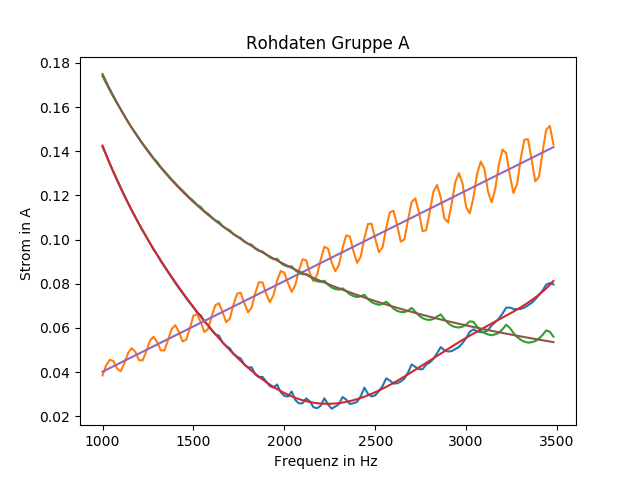
\includegraphics[scale=1]{Bilder/Parallel_Rohdaten.png}
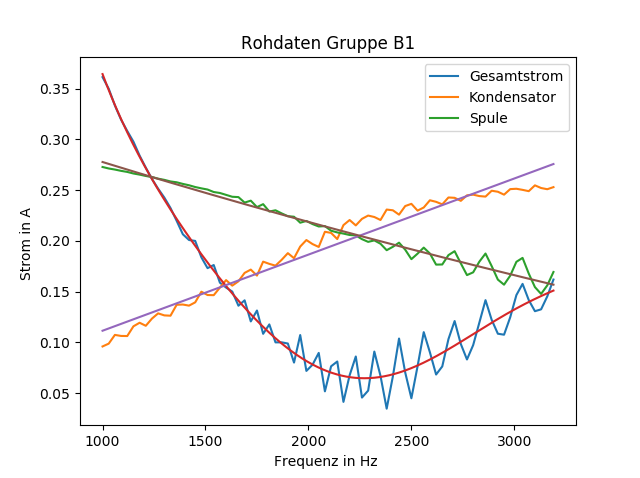
\includegraphics[scale=1]{Bilder/Parallel_RohdatenB.png}
\caption{Rohdaten des Gesamtstromes und der Ströme an Kondensator und Spule. Es wurden an die Daten Anpassungen durchgeführt, die versuchen, die Schwingung zu ignorieren.}
\label{fig:parallel_Rohdaten}
\end{figure}

Während der Durchführung wurde bei beiden Gruppen eine Periodische Schwankung in den gemessenen Strömen festgestellt. Dadurch gestaltet sich die Auswertung der Daten äußerst schwierig.\\
Deswegen wurde versucht, an die Rohdaten Anpassungen durchzuführen, die diese Schwingung ignorieren.\\
An den Gesamtstrom wurde wegen seiner recht komplizierten theoretischen Form ein Polynom 6. Grades, an den Kondensatorstrom eine lineare Funktion und an den Spulenstrom eine 1/x-Funktion angepasst.\\
Rohdaten und Anpassungen sind in Abbildung \ref{fig:parallel_Rohdaten} dargestellt.\\
Es ist zu erkennen, dass der Stromverlauf an Spule und Kondensator bei Gruppe B nicht wie erwartet verläuft. Es scheint dort ein Messfehler unterlaufen zu sein, weswegen diese Daten nicht weiter ausgewertet wurden.


\subsubsection{Bestimmung der Güte über den Gesamtstrom}
\begin{figure}
\centering
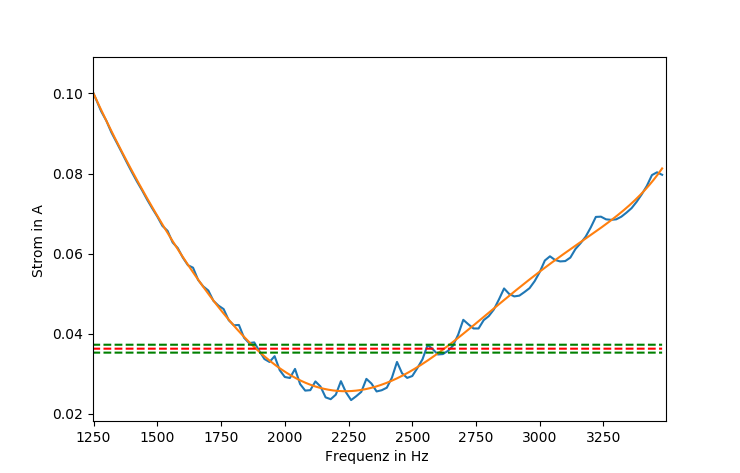
\includegraphics[scale=0.9]{Bilder/Parallel_Iges.png}
\caption{Bestimmung des Güte mithilfe des Gesamtstromes. Es wird zuerst das Minimum des Stromes bestimmt, das sich nahe der Resonanzfrequenz befindet. Dann wird geschaut, an welchen Stelle der Strom um $\sqrt{2}$ angestiegen ist (rote gestrichelte Linie) und daraus die Breite der Kurve bestimmt. Zur Fehlerabschätzung wird das Minimum um seinen Fehler verschoben und eine neue Breite abgeschätzt (grüne gestrichelte Linien). }
\label{fig:parallel_Iges}
\end{figure}

\begin{table}
\centering
\begin{tabular}{|c|c|c|c||c|c|}
\hline
Messung & A1 & A2 & A3 & B1 & B2\\
\hline
$f_0[Hz]$ & $2216\pm 23 $ & $2216\pm 29 $ & $2235\pm 17$ & $2272\pm 54$ & $2285\pm 55$\\
\hline
$\Delta f$ & $737\pm 19 $ & $488\pm 43 $ & $738\pm 24$ & $750\pm 81$ & $700\pm 79$\\
\hline
$Q$ & $3.01\pm 0.08 $ & $4.54\pm 0.41 $ & $3.03\pm 0.10$ & $3.03\pm 0.33$ & $3.26\pm 0.38$\\
\hline
\end{tabular}
\label{tab:parallel_methode1}
\caption{Ermittelte Daten aus der Gesamtstromkurve.}
\end{table}

Die Methode ist in Abbildung \ref{fig:parallel_Iges} dargestellt.
Mithilfe der Anpassung wurde der Minimale Gesamtstrom und damit $f_0$ bestimmt. Es macht wegen der Ungenauigkeit der Anpassung keinen Sinn einen Fehler aus dem Fit zu bestimmen.  Stattdessen wird der Fehler durch eine visuelle Abschätzung an den Rohdaten bestimmt.\\
Der Fehler auf den Wert des Stromes wird aus der Stärke der Schwankung bestimmt. Es macht keinen Sinn systematische Fehler zu betrachten, da die Werte durch die Schwankung nicht genau genug bestimmt werden können und der systematische Fehler wesentlich kleiner als der Ablesefehler ist.\\
Nun wird geschaut, an welchen Stellen der Strom um $\sqrt{2}$ angestiegen ist und aus dem Abstand von diesen Punkten $\Delta f$ berechnet.\\
Der Fehler folgt aus der Schwankung des Stromes. Dabei wird der Wert des Minimalen Stromes um seinen Fehler in beide Richtungen verschoben, ein neues $\Delta f$ für den verschobenen Wert berechnet und geschaut, wie weit der neue Wert vom alten abweicht.\\
Abschließend wird die Güte mithilfe von Formel ??? bestimmt.\\
Alle Ergebnisse sind in Tabelle \ref{tab:parallel_methode1} aufgelistet.\\
Eine gewichtete Mittelung der Messungen ergibtfür Gruppe A:
\begin{equation}
f_0 = \SI{2226(12)}{Hz}
\end{equation}
\begin{equation}
Q_A = 3.05\pm 0.17 
\end{equation}
und für Gruppe B:
\begin{equation}
f_0 = \SI{2278(39)}{Hz}
\end{equation}
\begin{equation}
Q_B = 3.13\pm 0.25 
\end{equation}
Dabei muss der äußere Fehler genommen werden.

\subsubsection{Bestimmung der Güte über Stromüberhöhung}
Bei dieser Auswertungsmethode wird die Resonanzfrequenz über den Schnittpunkt zwischen den Stromkurven von Spule und Kondensator ermittelt. Dieser kann direckt aus den Anpassungen bestimmt werden.\\
Da die Messwerte bei Gruppe B nicht dem erwarteten Verlauf folgen (vgl. Abbildung \ref{fig:parallel_Rohdaten}), wird diese Auswertung nur für Gruppe A durchgeführt.\\
Um einen Fehler auf den Wert zu bekommen, wird zuerst ein Fehler auf die gemessenen Ströme wie im vorherigen Kapitel abgeschätzt. Anschließend werden die Anpassungskurven um diesen Fehler verschoben und die neuen Schnittpunkte bestimmt. Der Fehler auf den Messwert beträgt dann die Hälfte des größten Abstandes zwischen zwei Schnittpunkten. Dises Verfahren wurde in Abbildung \ref{fig:parallel_Stromhoch} visualisiert.
Da der Wiederstand in der Spule wesentlich geringer ist als der benutzte Wiederstand ist, muss keine Korrekturrechnung durchgeführt werden.\\
Die somit bestimmten Schnittpunkt-Frequenzen sind in Tabelle \ref{tab:Stromhoch_Rohdaten} aufgelistet. Dort ist auch die Größe des Stromes am Kondensator und im gesamten Schwingkreis am Schnittpunkt zu finden. \\
Mithilfe von Gleichung \ref{eq:Parallel_Strmhoch} lässt sich daraus schließlich die Güte bestimmen. Es wurde der Strom an der Spule verwendet, da diser einen kleineren Fehler hat.

\begin{figure}
\centering
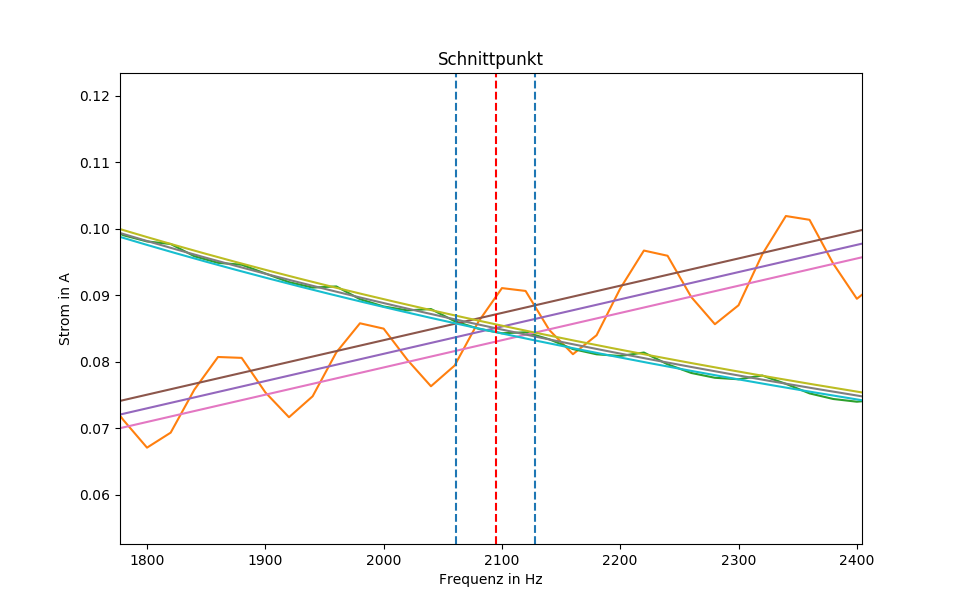
\includegraphics[scale=0.7]{Bilder/Parallel_Stromhoch.png}
\caption{Methode zur Bestimmung des Schnittpunktes (mittlere gestrichelte Linie) und seines Fehlers. Dazu werden die Stromkurven um ihre Fehler verschoben und die maximale Verschiebung des Schnittpunktes bestimmt.}
\label{fig:parallel_Stromhoch}
\end{figure}

\begin{table}
\centering
\begin{tabular}{|c|c|c|c|}
\hline
Messung & A1 & A2 & A3\\
\hline
$f_0[Hz]$ & $2094.6\pm 33.7$ & $2095.6\pm 38.2$ & $2093.7\pm 35.2$\\
\hline
$I_L$ & $0.0850\pm 0.0009$ & $0.1278\pm 0.0021$ & $0.1274\pm 0.0017$ \\
\hline
$I_0$ & $0.0256\pm 0.0009$ & $0.0234\pm 0.0029$ & $0.0390\pm 0.0018$ \\
\hline
$Q$ & $3.32\pm 0.11$ & $5.46\pm 0.50$ & $3.27\pm 0.15$ \\
\hline
\end{tabular}
\label{tab:Stromhoch_Rohdaten}
\caption{Gemessene Daten für die Resonanzfrequenz, der Stromstärken an Spule und im gesamten Schlatkreis bei der Resonanzfrequenz, sowie die daraus bestimmte Güte. Die Fehler folgen aus der in Abbildung \ref{fig:parallel_Stromhoch} beschriebenen Methode.}
\end{table}
Der gewichtete Mittelwert der ermittelten Güten beträgt mit äußerem Fehler:
\begin{equation}
Q = 3.37\pm 0.26 
\end{equation}

\subsubsection{Impedanz}
Aus
\begin{equation}
Z = \dfrac{U_{ges}}{I_{ges}}
\end{equation}
kann die Impedanz bestimmt werden. Diese sollte bei der Resonanzfrequenz maximal sein.\\
In Abbildung \ref{fig:parallel_Impedanz} ist die Impedanz beispielhaft dargestellt. Dabei wurde auch versucht eine Anpassung an diese Daten durchzuführen. Diese ist aber nicht gut genug gelungen, weswegen die Auswertung vollständig visuell gemacht wird.\\
In Tabelle \ref{tab:Parallel_Impedanz} sind die Resultate aufgelistet. Die Fehler wurden bestimmt, indem eine Gleichverteilung zwischen den zwei größten Messwerten angenommen wurde.\\
Daraus wurde wieder der gewichtete Mittelwert bestimmt:

\begin{equation}
Gruppe A: Z = \SI{52.7(81)}{\Omega}
\end{equation}

\begin{equation}
Gruppe B: Z = \SI{70.5(64)}{\Omega}
\end{equation}

\begin{table}
\centering
\begin{tabular}{|c|c|c|c||c|c|}
\hline
Messung & A1 & A2 & A3 & B1 & B2\\
\hline
$f_0[Hz]$ & $2218\pm 23$ & $2216\pm 23$ & $2219\pm 23$ & $2275\pm 30$ & $2275\pm 30$\\
\hline
$Z[\Omega]$ & $55\pm 3$ & $114\pm 29$ & $47\pm 4$ & $71\pm 9$ & $70\pm 9$\\
\hline
\end{tabular}
\label{tab:Parallel_Impedanz}
\caption{Ermittelte Daten bei der Messung an der Impedanzkurve. Die Fehler wurden visuell abgeschätzt und als gleichverteilt in diser Abschätzung angenommen.}
\end{table}

\begin{figure}
\centering
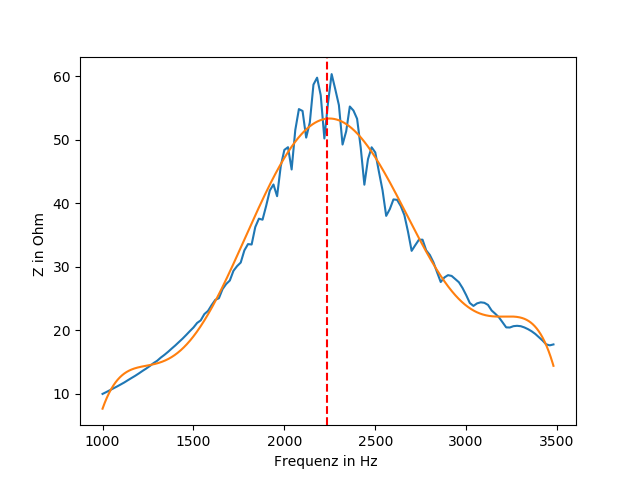
\includegraphics[scale=1]{Bilder/Parallel_Impedanz.png}
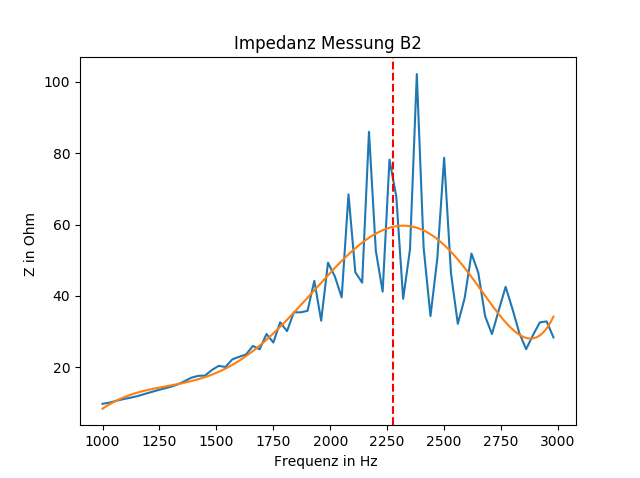
\includegraphics[scale=1]{Bilder/Parallel_ImpedanzB.png}
\caption{Impedanzverlauf von Gruppe A und B. Wegen der Schwankungen ist eine Anpassung an die Daten nicht geglückt. Die über das Minimum der Stromstärke bestimmte Resonanzfrequenz wurde mit einer senkrechten Linie makiert.}
\label{fig:parallel_Impedanz}
\end{figure}

\subsubsection{Phase}
\begin{figure}
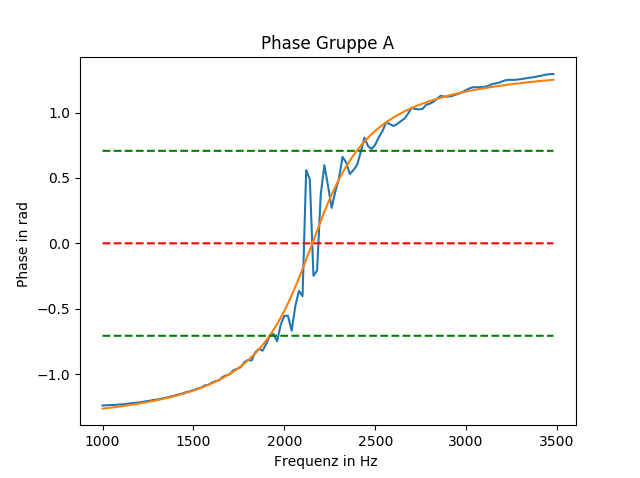
\includegraphics[scale=1]{Bilder/Parallel_Phase.png}
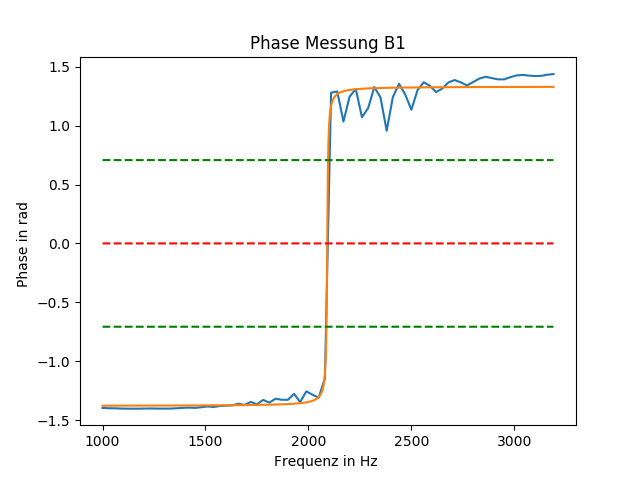
\includegraphics[scale=1]{Bilder/Parallel_PhaseB.png}
\caption{Phase zwischen Strom und Spannung der Messreihe 1. An die Rohdaten wurde eine Arcustangens-Funktion angepasst. Es wurden außerdem die Winkel $0^\circ, 45^\circ und -45^\circ$ durch gestrichelte Linien markiert.}
\label{fig:parallel_Phase}
\end{figure}

Aus der Phase Zwischen Strom und Spannung kann auch hier die Resonanzfreqenz bestimmt werden, bei der die Phase 0 beträgt.\\
In Abbildung \ref{fig:parallel_Phase} ist die Phasenbeziehung beispielhaft gezeigt. Auch hier ist offensichtlich wieder eine störende Schwingung vorhanden. Um die Daten besser auswerten zu können wird eine arcustangens-Funktion an die Daten angepasst. An dieser wird dann die Nullstelle abgelesen.
Die Fehler werden visuell abgeschätzt.\\
Die so bestimmten Resonanzfrequenzen sind in Tabelle  \ref{tab:Parallel_Phase} aufgelistet.

\begin{table}
\centering
\begin{tabular}{|c|c|c|c||c|c|}
\hline
Messung & A1 & A2 & A3 & B1 & B2\\
\hline
$f_0[Hz]$ & $2154\pm 42$ &$ 2137\pm 30$ & $2137\pm 32$ & $2094\pm 16$ & $2094\pm 16$\\
\hline
\end{tabular}
\caption{Abgeschätzte Resonanzfrequenzen aus der Phasendifferenz zwischen Spannung und Strom. Die Fehler wurden visuell abgeschätzt.}
\label{tab:Parallel_Phase}
\end{table}

Aus diesen wird abschließend noch der gewichtete Mittelwert gebildet:
\begin{equation}
Gruppe A: f_0 = \SI{2141(19)}{Hz}
\end{equation}

\begin{equation}
Gruppe B: f_0 = \SI{2094(11)}{Hz}
\end{equation}

\subsection{Zusammenfassung}

\begin{table}[h]
\centering
\begin{tabular}{|c|c|c|c|c|c|}
\hline
Wert & Gesamtstrom & Stromüberhöhung & Impedanz & Phase & Erwartungswert\\
\hline
\hline
$f_0[Hz]$ & $2226\pm 12$ &$ 2095\pm 12$ & $2218\pm 27$ & $2141\pm 19$ & $2076$\\
\hline
$\sigma$ & $12.5$ & $1.6$ & $5.3$ & $3.4$ & -\\
\hline
\hline
$Q$ & $3.05\pm 0.17$ &$ 3.37\pm 0.26$ & - & - & $4.63$\\
\hline
$\sigma$ & $9.2$ & $4.8$ & - & - & -\\
\hline
\hline
$Z[\Omega]$ & - & - & $52.7\pm 8.1$ & - & $347$\\
\hline
$\sigma$ & - & - & $36.3$ & - & -\\
\hline
\end{tabular}
\caption{Zusammenfassung aller Ergebnisse von Gruppe A. Es wurde zu allen Werten die Standardabweichungen vom Literaturwert angegeben.}
\label{tab:Parallel_FazitA}
\end{table}

\begin{table}[h]
\centering
\begin{tabular}{|c|c|c|c|c|}
\hline
Wert & Gesamtstrom & Impedanz & Phase & Erwartungswert\\
\hline
\hline
$f_0[Hz]$ & $2278\pm 39$ & $2275\pm 21$ & $2094\pm 11$ & $0$\\
\hline
$\sigma$ & $12.5$ & $5.3$ & $3.4$ & -\\
\hline
\hline
$Q$ & $3.13\pm 0.25$ &  - & - & $0$\\
\hline
$\sigma$ & $9.2$ &  - & - & -\\
\hline
\hline
$Z[\Omega]$ - & $70.5\pm 6.4$ & - &  - &$0$\\
\hline
$\sigma$ & - & $36.3$ & - & -\\
\hline
\end{tabular}
\caption{Zusammenfassung aller Ergebnisse von Gruppe B. Es wurde zu allen Werten die Standardabweichungen vom Literaturwert angegeben.}
\label{tab:Parallel_FazitB}
\end{table}

Die Erwartungswerte der Messgrößen wurden folgendermaßen aus den Bauteilen des Schwingkreises bestimmt:
\begin{equation}
f_0 = \sqrt{\dfrac{1-\frac{C}{L}\cdot R_L^{2}}{LC}}\cdot \dfrac{1}{2\pi}
\end{equation}
\begin{equation}
Q = \dfrac{R\cdot \sqrt{\frac{C}{L}}}{1+R\cdot R_L\cdot \frac{C}{L}}
\end{equation}
\begin{equation}
Z_{res} = \dfrac{L}{C\cdot R_L}
\end{equation}

In Tabelle \ref{tab:Parallel_FazitA} und \ref{tab:Parallel_FazitB} sind nochmal alle ausgewerteten Messgrößen aufgelistet.\\
Dort sind außerdem die Abweichungen vom Erwartungswert angegeben, der aus den Komponenten des Schwingkreises bestimmt wurde.\\
Die ermittelten Werte für die Resonanzfrequenz schwanken zwischen den verschiedenen Verfahren um mehr als 150 Hz und liegen bis zu 12 Standardabweichungen vom Erwartungswert entfernt. Da die Verfahren theoretisch aber nur in der Näherung übereinstimmen war diese Abweichung zu erwarten.\\
Die experimentell bestimmten Güten weichen zwar auch um bis zu 35\% vom Erwartungswert ab, stimmen aber innerhalb ihrer Abweichung miteinander überein. Die großen Fehler von bis zu 8\% sind auf die unbekannte Systematik zurückzuführen, die das Bestimmen der Werte sehr schwierig gemacht hat.



\newpage
\section{Hoch- und Tiefpass}

In diesem Versuch soll die Übertragsfunktion von Hoch- bzw. Tiefpass aufgezeichnet werden und die charakteristische Frequenz $\omega_0$ des Aufbaus bestimmt werden.

\subsection{Auf und Durchführung}

\begin{figure}
\centering
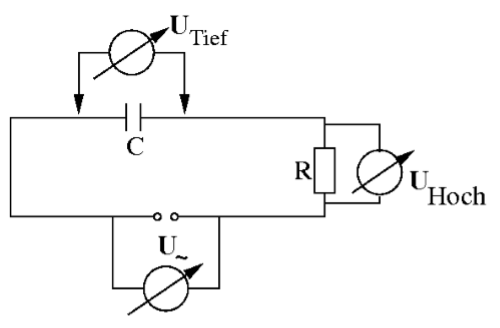
\includegraphics[scale=1.0]{Bilder/AufbauHochTief.png}
\caption{Schaltskizze zum Hoch- bzw Tiefpass. (Quelle: Praktikumsskript S. 94)}
\label{fig:AufbauHochTief}
\end{figure}

Der Versuchsaufbau erfolgt nach der Schaltskizze in Abbildung \ref{fig:AufbauHochTief}. Die Spannungen an Widerstand und Kondensator
werden mit dem Sensor-CASSY aufgezeichnet. Die Spannungsquelle ist erneut durch das Power-CASSY gegeben, welches gleichzeitig die angelegte Spannung misst. Alle Messwerte werden als Effektivwerte gemessen.

Die Frequenz wird wieder automatisch schrittweise bis zu einem maximalen Wert erhöht. Die Einstellungen diesbezüglich sind identisch zu den vorherigen Versuchen. Die Wechselspannungsamplitude wurde zu 5V eingestellt.

Gruppe A verwendet in ihrem Aufbau den $\SI{4,7}{\micro \F}$ Kondensator und den $\SI{100}{\ohm}$ Widerstand. Gruppe B hat einen Kondensator mit gleichem Nominalwert und einen $\SI{10}{\ohm}$ Widerstand benutzt.

\subsection{Auswertung}

\begin{figure}
\centering
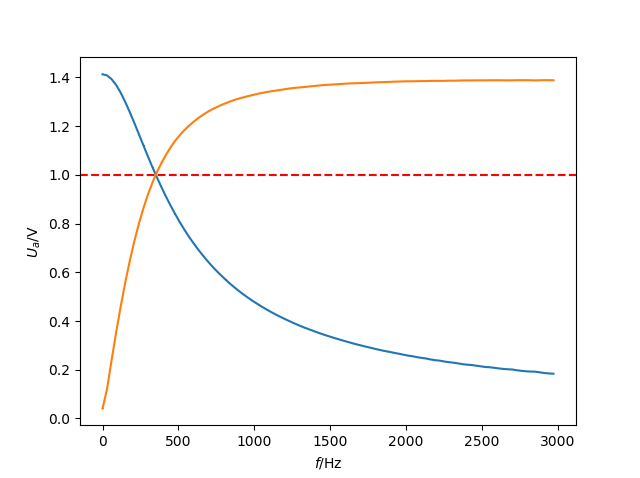
\includegraphics[scale=1.0]{Bilder/RohdatenHochTief_A.png}
\caption{Rohdaten für Gruppe A. eine Hilfslinie bei $\frac{U_{eff}}{\sqrt{2}}$, wobei $U_{eff}$ der Effektivwert der angelegten Spannung ist, eingezeichnet.}
\label{fig:RohdatenHochTief_A}
\end{figure}

\begin{figure}
\centering
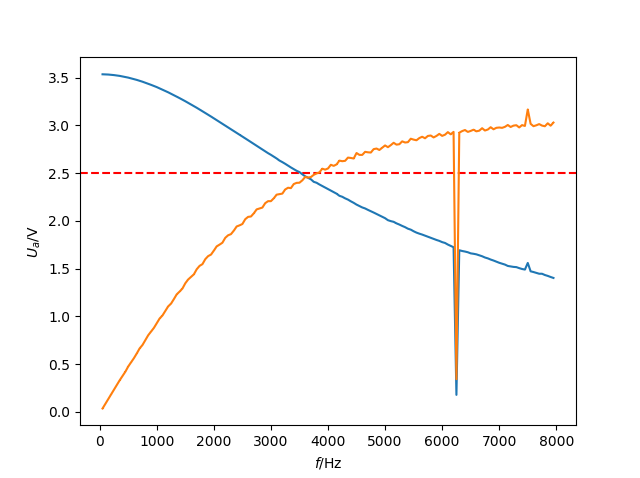
\includegraphics[scale=1.0]{Bilder/RohdatenHochTief_B.png}
\caption{Rohdaten der aufgezeichneten Spannungen für Gruppe B. Es sind Hilfslinien bei $U_{eff}$ und $\frac{U_{eff}}{\sqrt{2}}$, wobei $U_{eff}$ der Effektivwert der angelegten Spannung ist, eingezeichnet.}
\label{fig:RohdatenHochTief_B}
\end{figure}

Die Rohdaten der Versuche finden sich in den Abbildungen \ref{fig:RohdatenHochTief_A} und \ref{fig:RohdatenHochTief_B}.

Zur Bestimmung Der charakteristischen Frequenz wird der Schnittpunkt der Spannungsverläufe mit der Geraden $\frac{U_{eff}}{\sqrt{2}}$ bestimmt (vgl. Gleichungen \ref{equ:Hochpass} und \ref{equ:Tiefpass}).

Der Schnittpunkt wird unter Berücksichtigung des statistischen Fehlers auf die Spannungsmessung abgelesen. Dabei ergibt sich durch die Ablesegenauigkeit ein statistischer Fehler auf die so bestimmten Frequenzen.
Zur Berücksichtigung der systematischen Fehler werden zunächst die Offsets korrigiert. Die "linearen" systematischen Fehler werden auf die Spannungsmessung addiert bzw. abgezogen. 
Die Frequenzbestimmung wird an den verschobenen Kurven erneut vorgenommen. Der Abstände zwischen Frequenz der unveränderten Kurve und den Frequenzen der verschobenen Kurven stellen den systematischen Fehler dar. Durch die Herstellerangabe von $\sigma_{U_i} = 0,01 \cdot U_i$ ist dieser relativ groß.

Eine alternative Möglichkeit zur Bestimmung der charakteristischen Frequenz ist durch die Phase zwischen den Spannungen gegeben. Bei erreichen der charakteristischen Frequenz beträgt die Phasendifferenz $\ang{45}$. Die Phase wird vom CASSY intern gemessen und es liegen keine Informationen zur Art und Weise der Bestimmung vor. Es kann somit nur ein statistischer Ablesefehler bei der Frequenzbestimmung angenommen werden. Der Verlauf der Phase für beide Gruppen findet sich in Abbildung \ref{fig:HochTiefPhase}.

Als Vergleichswert kann auch die theoretische Erwartung über $f = \frac{1}{2\pi RC}$ berechnet werden. Die Werte von R und C wurden durch die Brücke im Raum bestimmt, wobei eine statistische Unsicherheit auf die letzte Stelle und eine systematische Unsicherheit von $0,25$\% angenommen wurden. Für Gruppe A ergab sich $R=\SI{99,08}{\ohm}$ und $C=\SI{4,597}{\micro \F}$, für Gruppe B $R=\SI{9,988}{\ohm}$ und $C=\SI{4,475}{\micro \F}$. Mittels Fehlerfortpflanzung ergibt folgt:

\begin{equation}
\sigma_f = f \sqrt{\left( \frac{\sigma_R}{R} \right)^2+\left( \frac{\sigma_C}{C} \right)^2}
\end{equation}

Die auf die verschiedenen Arten bestimmten charakteristischen Frequenzen befinden sich in Tabelle \ref{tab:HochTief}.

\begin{figure}
\centering
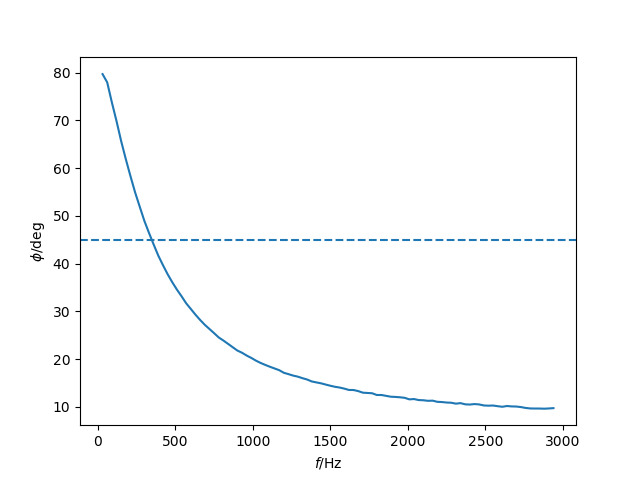
\includegraphics[scale=0.5]{Bilder/PhaseHochTief_A.png}
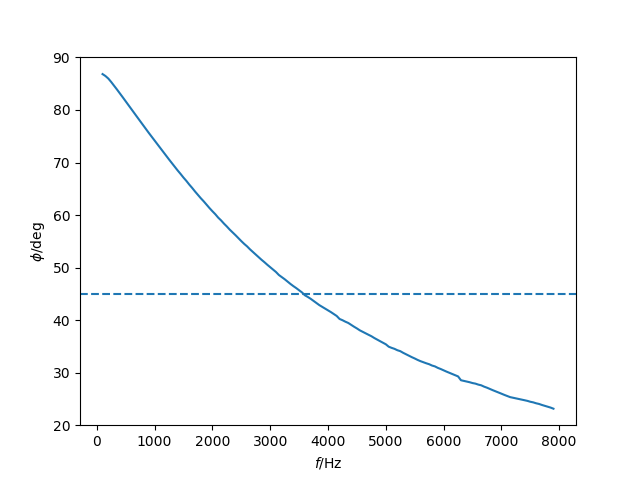
\includegraphics[scale=0.5]{Bilder/PhaseHochTief_B.png}
\caption{Phasenverschiebungen für Gruppe A (links) und Gruppe B (rechts).}
\label{fig:HochTiefPhase}
\end{figure}


\begin{table}
\centering
\begin{tabular}{|c|c|c|c|c|}
\hline
Gruppe & $f_{Tiefpass}$ & $f_{Hochpass}$ & $f_{Phase}$ &  $f_{Erwartung}$ \\
\hline
A & $(352 \pm 3 \substack{+7\\-8})$Hz & $(350 \pm 3 \pm 7)$Hz & $(347 \pm 6)$Hz & $(349,43 \pm 0,08 \pm 1,22)$Hz \\
\hline
B & $(3524 \pm 16 \substack{+44 \\ -91})$Hz & $(3815 \pm 10 \substack{+37 \\ -165})$Hz & $(3577 \pm 15)$Hz & $(3561 \pm 1 \pm 12)$Hz \\
\hline
\end{tabular}
\caption{Abgelesene Frequenzen mitsamt abgeschätztem statistischen und, falls vorhanden, systematischen Fehler für beide Gruppen.}
\label{tab:HochTief}
\end{table}

\paragraph{Fazit} \mbox{}\\
Unter Berücksichtigung der Fehler sind die Ergebnisse von Gruppe A mit Abweichungen von weniger als einer Standardabweichung untereinander konsistent. Auch eine ebenso gute Übereinstimmung zur theoretischen Erwartung, die aus den Bauteilen berechnet wurde, ist gegeben.

Bei Gruppe B ist die Übereinstimmung von theoretischer Erwartung und Bestimmung durch die Phasenverschiebung im Rahmen der Fehler vereinbar. Besonders auffällig sind hier allerdings die sehr großen, unsymmetrischen, systematischen Fehler von bis zu 5\%. Zwar sind ist die systematische Spannungsunsicherheit mit 1\% deutlich kleiner, bei Übersetzung in eine Frequenzunsicherheit durch die Verschiebung kommt es allerdings aufgrund des Kurvenverlaufs zu dieser Vergrößerung des Fehlers. Zwar läge die theoretische Erwartung noch innerhalb der Unsicherheit von $f_{Tiefpass}$ und $f_{Hochpass}$, die Bestimmung an sich ist wegen der großen systematischen Unsicherheiten dennoch ungenau.




\end{document}